% Tutorial set: 06
% Source: tute6.pdf, PDF pp. 1--2, Questions 1--3
% Reference: tute6_ans.pdf, PDF pp. 2--24
% Session date: 2026-09-23
% Q1 numerically recomputed; Q2/Q3 reference experiments explained, not rerun.

\exercisegroup{SC4001-TUT06}{Tutorial 06：Convolutional Neural Networks}
\label{tutorial:SC4001-TUT06}
\exercisemeta
  {SC4001-TUT06}
  {2026-09-23}
  {\texttt{tute6.pdf} pp.~1--2，Q1--Q3；\texttt{tute6\_ans.pdf} pp.~2--24}
  {Q1 数值已复算；Q2、Q3 参考实验已分析，未重新训练}
  {已请求整理笔记（2026-09-23）}

题目页眉沿用旧代码 CZ4042，参考答案封面标注 SC4001。本组围绕卷积计算、多通道特征图和 CNN 分类；实验图片均为参考答案中的结果，不是独立复现。

\exercisequestion{SC4001-TUT06-Q01}{卷积、Sigmoid 与两种 Pooling}
\textbf{对应讲义：}\relatedtopic{SC4001-L06-T02}{卷积尺寸与运算}；\relatedtopic{SC4001-L06-T03}{Activation 与 Pooling}。

\subsubsection*{题目与约定（题目 p.~1；答案 pp.~2--11）}
输入为单通道 $6\times6$ 图像，两个 $3\times3$ filters（卷积核），各自 bias（偏置）均为 $0.1$，激活函数为 sigmoid：
\[
I=\begin{pmatrix}
0.7&0.1&0.2&0.3&0.3&0.5\\
0.8&0.1&0.3&0.5&0.1&0.0\\
1.0&0.2&0.0&0.3&0.2&0.7\\
0.8&0.1&0.5&0.6&0.3&0.4\\
0.1&0.0&0.9&0.3&0.3&0.2\\
1.0&0.1&0.4&0.5&0.2&0.8
\end{pmatrix},\quad
W_1=\begin{pmatrix}0&1&1\\1&0&1\\1&1&0\end{pmatrix},\quad
W_2=\begin{pmatrix}-1&-1&-1\\0&0&0\\1&1&1\end{pmatrix}.
\]
(a) 分别求 padding $P=0$、stride $S=1$，以及 $P=1$、$S=2$ 的卷积层输出；(b) 对两种输出分别做 $2\times2$、stride $2$ 的 max pooling（最大池化）与 mean pooling（平均池化）。池化按答案采用 VALID、不补零。原题右上角的 ``05'' 按答案展开计算中的 $0.5$ 处理。

\begin{checkedsolution}
\textbf{计算顺序。}沿用 CNN 的 cross-correlation（互相关）约定，不翻转卷积核：
\[
u_k(i,j)=\sum_{r,c}W_k(r,c)\,I_{\mathrm{window}}(r,c)+0.1,
\qquad y_k(i,j)=\sigma(u_k(i,j))=\frac1{1+e^{-u_k(i,j)}}.
\]
每个核生成一张 feature map（特征图），偏置在每个输出位置只加一次。池化逐通道作用于 $y_k$，不作用于 $u_k$，也不混合两个通道。输出边长为
\[
N_{\mathrm{out}}=\left\lfloor\frac{N+2P-K}{S}\right\rfloor+1.
\]
\begin{center}
\begin{tabular}{@{}lcc@{}}
\toprule
卷积设置 & 每张卷积输出 & 每张池化输出 \\
\midrule
$P=0,S=1$ & $4\times4$ & $2\times2$ \\
$P=1,S=2$ & $3\times3$ & $1\times1$ \\
\bottomrule
\end{tabular}
\end{center}

\textbf{(a-i) 不补零、stride 为 1。}左上角窗口给出
\[
u_1(1,1)=0.1+0.2+0.8+0.3+1.0+0.2+0.1=2.7,
\]
\[
u_2(1,1)=-(0.7+0.1+0.2)+(1.0+0.2+0.0)+0.1=0.3.
\]
其余位置同理，完整 pre-activation（激活前输入）为
\[
u_1=\begin{pmatrix}2.7&1.4&1.4&1.9\\2.4&2.0&2.0&2.1\\1.7&2.0&2.6&2.6\\2.8&2.0&3.1&2.0\end{pmatrix},\qquad
u_2=\begin{pmatrix}0.3&0.0&-0.2&0.2\\0.3&0.4&0.6&0.8\\-0.1&0.8&1.1&-0.3\\0.2&-0.1&-0.2&0.3\end{pmatrix}.
\]
卷积层的实际输出为
\[
y_1\approx\begin{pmatrix}.9370&.8022&.8022&.8699\\.9168&.8808&.8808&.8909\\.8455&.8808&.9309&.9309\\.9427&.8808&.9569&.8808\end{pmatrix},\quad
y_2\approx\begin{pmatrix}.5744&.5000&.4502&.5498\\.5744&.5987&.6457&.6900\\.4750&.6900&.7503&.4256\\.5498&.4750&.4502&.5744\end{pmatrix}.
\]
\textbf{勘误：}答案 p.~4 将 $u_2(1,4)$ 写成 $2.0$，正确为 $0.2$；该页给出的 $y_2(1,4)\approx0.55$ 则与正确值一致。

\textbf{(a-ii) 四周补一圈零、stride 为 2。}第一个窗口为
\[
\begin{pmatrix}0&0&0\\0&0.7&0.1\\0&0.8&0.1\end{pmatrix},
\qquad u_1(1,1)=0.1+0.8+0.1=1.0.
\]
窗口随后沿行、列每次移动两格，得到
\[
u_1=\begin{pmatrix}1.0&0.9&1.5\\2.0&2.0&2.1\\2.0&2.0&2.0\end{pmatrix},\qquad
u_2=\begin{pmatrix}1.0&1.0&0.7\\0.1&0.4&0.8\\0.3&-0.1&0.3\end{pmatrix},
\]
\[
y_1\approx\begin{pmatrix}.7311&.7109&.8176\\.8808&.8808&.8909\\.8808&.8808&.8808\end{pmatrix},\qquad
y_2\approx\begin{pmatrix}.7311&.7311&.6682\\.5250&.5987&.6900\\.5744&.4750&.5744\end{pmatrix}.
\]

\textbf{(b) 池化结果。}以下 $M_k,A_k$ 分别表示第 $k$ 个通道的 max、mean pooling。对 (a-i) 的 $4\times4$ 特征图：
\[
M_1\approx\begin{pmatrix}.9370&.8909\\.9427&.9569\end{pmatrix},\qquad
M_2\approx\begin{pmatrix}.5987&.6900\\.6900&.7503\end{pmatrix},
\]
\[
A_1\approx\begin{pmatrix}.8842&.8609\\.8875&.9249\end{pmatrix},\qquad
A_2\approx\begin{pmatrix}.5619&.5839\\.5475&.5501\end{pmatrix}.
\]
例如 $A_1(1,1)$ 是 $y_1$ 左上角四个值的平均，计算时使用未舍入的 sigmoid 数值。对 (a-ii) 的 $3\times3$ 特征图：
\[
M_1\approx(.8808),\quad M_2\approx(.7311),\qquad
A_1\approx(.8009),\quad A_2\approx(.6464).
\]
此时只有左上角 $2\times2$ 窗口放得下，最后一行、最后一列不会参与池化；不是把九个数合为一个。Max pooling 保留局部最强响应，mean pooling 保留局部平均响应。特别注意
\[
\operatorname{mean}(\sigma(u))\ne\sigma(\operatorname{mean}(u))
\]
一般不能交换激活与平均；两种池化均不改变通道数。
\end{checkedsolution}

\exercisequestion{SC4001-TUT06-Q02}{RGB 图像：多通道卷积与平均池化}
\textbf{对应讲义：}\relatedtopic{SC4001-L06-T01}{Feature Maps}；\relatedtopic{SC4001-L06-T02}{多通道卷积与参数}。

\subsubsection*{题目（题目 p.~1；答案 pp.~12--16）}
对 $639\times516$ 的彩色图像 \texttt{3wolfmoon.jpg}：
(a) 初始化一个含两个 $9\times9$ kernels 的卷积层的权重与偏置；
(b) 使用 sigmoid、VALID padding、stride $1$，显示卷积 feature maps；
(c) 使用 $5\times5$、stride $5$ 的 mean pooling，显示输出。

\begin{workedsolution}
\textbf{RGB 的合并方式。}每个核实际包含三个通道，形状为 $3\times9\times9$：
\[
u_k(i,j)=\sum_{c=1}^3\sum_{r,s}W_{k,c,r,s}I_{c,i+r,j+s}+b_k,
\qquad y_k=\sigma(u_k),\quad k=1,2.
\]
三个颜色通道的加权贡献求和后才加偏置、做激活；一个核产生一张图，不是每个颜色各产生一张最终图。卷积层共 $2(3\times9\times9+1)=488$ 个可学习参数。

\textbf{形状与初始化。}按参考图的高、宽顺序，采用 $H\times W\times C$ 记法：
\begin{gather*}
639\times516\times3
\xrightarrow[\text{stride }1]{9\times9\ \mathrm{conv}+\mathrm{sigmoid}}
631\times508\times2,\\
631\times508\times2
\xrightarrow[\text{stride }5]{5\times5\ \mathrm{mean\ pool}}
126\times101\times2.
\end{gather*}
两层均采用 VALID；池化边长例如 $\lfloor(631-5)/5\rfloor+1=126$。
题目没有规定初始化分布或 seed，所以输出像素没有唯一数值答案。一种可行实现是小幅随机权重、零偏置，输入统一缩放后再前向计算；这是实现建议，不是对参考 notebook 设置的断言。复现时还应记录输入缩放、随机种子与各层参数。

\begin{figure}[H]
\centering
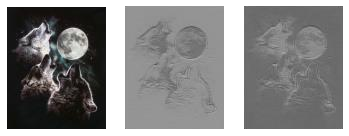
\includegraphics[width=.66\textwidth]{figures/source/tutorial-06-rgb-conv.png}
\caption{从左至右：RGB 原图、卷积特征图 1、卷积特征图 2。来源：\texttt{tute6\_ans.pdf} p.~15 的图像区域；原始图像分辨率较低，未重新生成实验结果。}
\label{fig:sc4001-tut06-rgb}
\end{figure}
不同核强调不同的局部亮度、颜色或轮廓组合；随后平均池化保留较粗的空间响应、减少细节。本题只要求初始化与前向显示，没有识别目标或训练步骤，因此不能把这些图解释为网络已学会“识别狼”。
\end{workedsolution}

\exercisequestion{SC4001-TUT06-Q03}{MNIST CNN：训练曲线、权重与特征图}
\textbf{对应讲义：}\relatedtopic{SC4001-L06-T04}{CNN 分类头}；\relatedtopic{SC4001-L06-T05}{训练流程}；\relatedtopic{SC4001-L06-T06}{SGD 与 Momentum}。

\subsubsection*{题目（题目 pp.~1--2；答案 pp.~17--24）}
设计一个卷积隐藏层识别 MNIST：使用 $25$ 个 $9\times9$ 卷积核、$4\times4$ 池化窗口、VALID padding 和默认 strides。用 mini-batch gradient descent（小批量梯度下降）训练，学习率 $\alpha=10^{-3}$，batch size 为 $128$。
要求：(a) 画 training/test errors 随 epoch 的曲线；(b) 显示最终卷积核权重；(c) 对一个代表性测试样本显示卷积层、池化层特征图；(d) 加入 decay $\beta=10^{-6}$ 和 momentum $\gamma=0.5$，重新训练并比较学习曲线。

\begin{workedsolution}
\textbf{网络与数据。}答案使用 $60\,000$ 张训练图像、$10\,000$ 张测试图像，均为 $28\times28$ 灰度图。按 p.~19 的结构，卷积 stride 为 $1$、池化 stride 为 $4$：
\begin{gather*}
\underbrace{1\times28\times28}_{\text{输入}}
\xrightarrow{9\times9\ \mathrm{conv}+\mathrm{ReLU}}
\underbrace{25\times20\times20}_{\text{卷积特征图}}
\xrightarrow{4\times4\ \mathrm{pool}}
\underbrace{25\times5\times5}_{\text{池化特征图}},\\
25\times5\times5\xrightarrow{\mathrm{flatten}}625
\xrightarrow{\mathrm{FC}+\mathrm{softmax}}10\text{ 类概率}.
\end{gather*}
此处尺寸为 $C\times H\times W$；flatten 只展平数据，没有可学习参数。
“一个隐藏层”指这里的卷积特征提取结构，仍有最终分类层。\verify{两份 PDF 未明确 Q3 的池化是 max 还是 mean；没有 notebook，不能确认。}
作为实现补充，若使用 \texttt{CrossEntropyLoss}，FC 应输出 raw logits 直接计算损失；Softmax 用于解释预测概率，不应在该损失之前重复应用。

\textbf{(a) 学习曲线的评价口径。}答案 p.~20 只展示 test accuracy，不是题目要求的完整训练、测试误差曲线。分类错误率满足 $e=1-\mathrm{accuracy}$（准确率以 $[0,1]$ 表示），但交叉熵并不等于 $1-\mathrm{accuracy}$。参考普通梯度下降运行在约 $50$ 个 epoch 后达到约 $76\%$--$77\%$ 的 test accuracy；这是图上读数，不是该架构的性能上限。没有训练曲线，不能单凭它判断训练与测试的差距或断言过拟合。

\textbf{(b)(c) Filter 与 Feature Map。}图~\ref{fig:sc4001-tut06-maps} 对比卷积参数、数字 9 的卷积响应及池化响应：
\begin{figure}[H]
\centering
\begin{minipage}{.31\textwidth}\centering
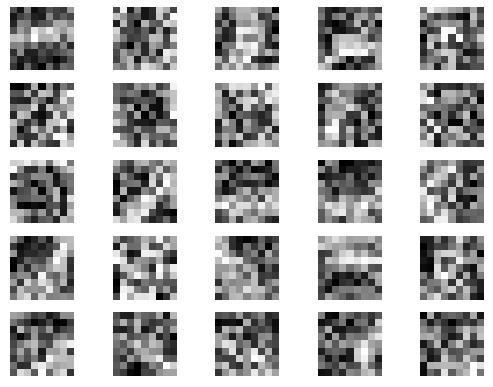
\includegraphics[width=\linewidth]{figures/source/tutorial-06-filters.png}\\
{\small 25 个 $9\times9$ filters}
\end{minipage}\hfill
\begin{minipage}{.31\textwidth}\centering
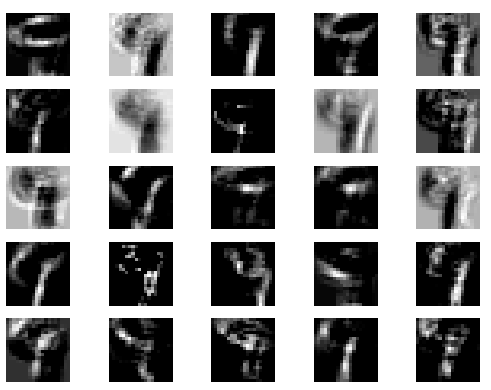
\includegraphics[width=\linewidth]{figures/source/tutorial-06-conv-maps.png}\\
{\small 25 张 $20\times20$ 特征图}
\end{minipage}\hfill
\begin{minipage}{.31\textwidth}\centering
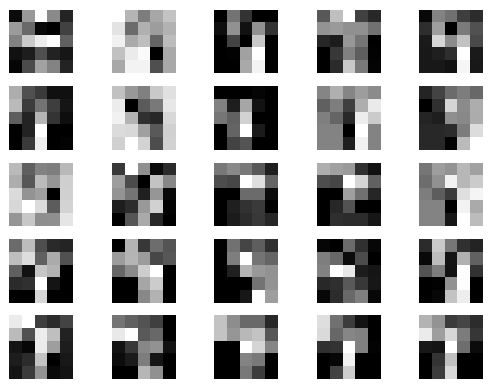
\includegraphics[width=\linewidth]{figures/source/tutorial-06-pool-maps.png}\\
{\small 25 张 $5\times5$ 池化图}
\end{minipage}
\caption{参考实验的参数与激活可视化。来源：\texttt{tute6\_ans.pdf} p.~23 的 filters，p.~22 的 convolution/pooling maps；输入为数字 9。仅提取图像，非本次训练。}
\label{fig:sc4001-tut06-maps}
\end{figure}
Filter 是训练得到的参数，训练结束后换输入不会改变它；feature map 是特定输入的响应，换输入就会变化。不同核对笔画、弯曲或局部边缘的响应不同；池化使位置表示更粗，但保留部分强响应区域。$25$ 个核不代表 $25$ 个类别，也不要求每个核都可命名为一个明确的语义检测器。图像按显示尺度映射为灰度，不能仅凭黑白判断不同图的绝对数值大小。

\textbf{(d) Weight Decay 与 Momentum。}采用一致的 L2 系数约定：
\[
J_{\mathrm{reg}}(W,b)=J(W,b)+\frac\beta2\lVert W\rVert_F^2,
\qquad \nabla_WJ_{\mathrm{reg}}=\nabla_WJ+\beta W.
\]
普通 SGD 加 decay 时，
\[
W_{t+1}=(1-\alpha\beta)W_t-\alpha\nabla_WJ(W_t,b_t).
\]
Weight decay 给权重向零收缩的倾向，不是 learning-rate decay（学习率衰减）。Momentum 保留上次更新方向；合并两者并令 $V_0=0$，得到
\[
V_{t+1}=\gamma V_t-\alpha\bigl(\nabla_WJ(W_t,b_t)+\beta W_t\bigr),
\qquad W_{t+1}=W_t+V_{t+1}.
\]
梯度方向持续一致时动量可积累，摆动方向则可部分抵消。这里的正则项只写权重 $W$；不能自行断言参考实现也惩罚了 bias。答案 p.~24 使用 $\beta_2\sum_{ij}W_{ij}^2$ 表示惩罚项，若更新用 $\beta W$，系数应满足 $\beta=2\beta_2$。

\begin{figure}[H]
\centering
\begin{minipage}{.48\textwidth}\centering
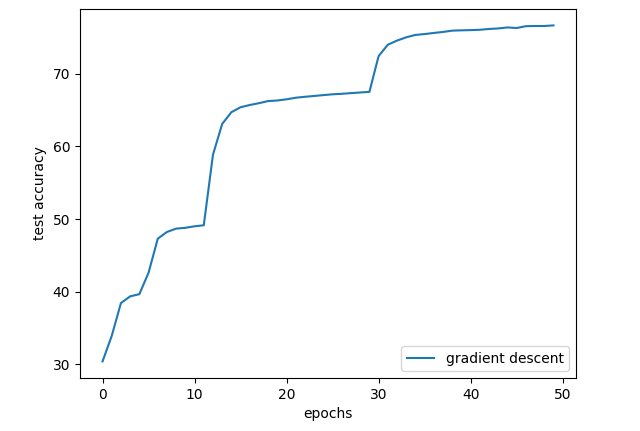
\includegraphics[width=\linewidth]{figures/source/tutorial-06-sgd.png}\\
{\small 普通梯度下降}
\end{minipage}\hfill
\begin{minipage}{.48\textwidth}\centering
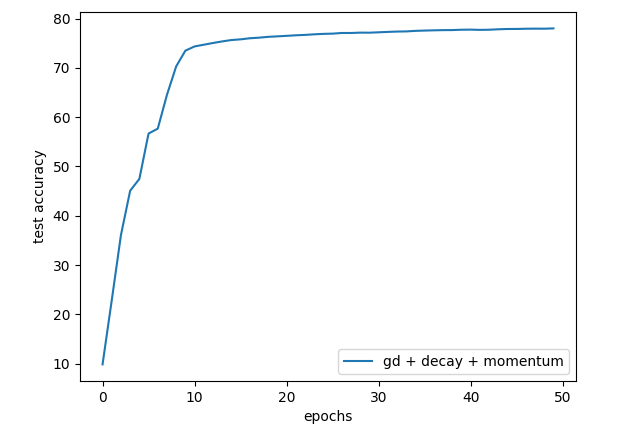
\includegraphics[width=\linewidth]{figures/source/tutorial-06-momentum-decay.png}\\
{\small 加入 decay 与 momentum}
\end{minipage}
\caption{两次参考运行的 test accuracy。来源：\texttt{tute6\_ans.pdf} p.~24；保留原始坐标刻度，两图纵轴下界不同。}
\label{fig:sc4001-tut06-curves}
\end{figure}
加入两者的参考曲线更早达到约 $75\%$，最终约 $78\%$，主要展示达到较高准确率所需 epoch 减少；不是普遍性能保证。由于同时改变 decay 和 momentum，不能单独归因于其中之一；若要分离作用，需保持其他条件一致并分别比较。

\textbf{评价边界。}应记录初始化、数据处理、优化器与运行配置；如需调参或选 epoch，使用 validation set（验证集），不能反复利用测试曲线做选择。参考 PDF 没有提供完整训练曲线、日志和 notebook 内容，本组仅解释已展示的实验，未补造缺失结果。
\end{workedsolution}
